\chapter{Grobentwurf}
\\[\intextsep]
\begin{minipage}{\linewidth}
\centering%
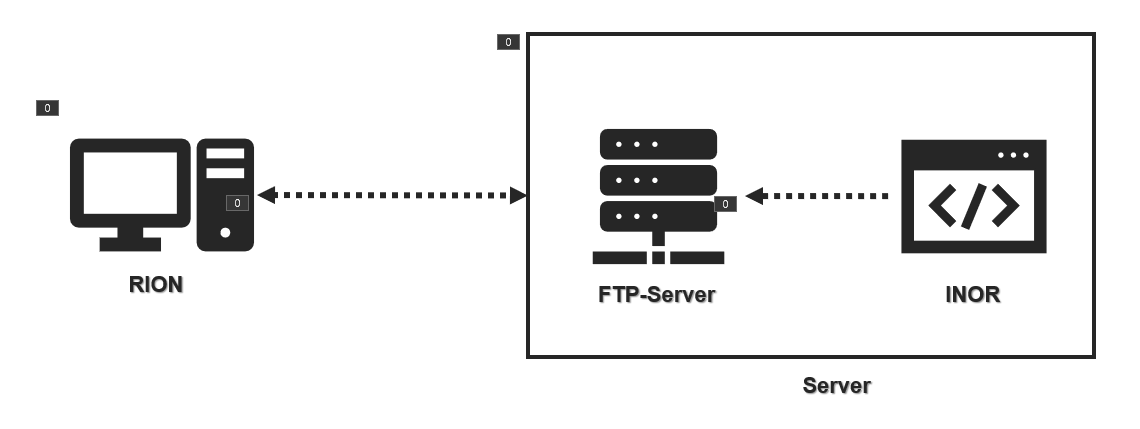
\includegraphics[width=0.8\linewidth,clip=]{./img/Img1.jpg}%
\label{fig:Image 1}%
\end{minipage}
\\[\intextsep]

Das Programm arbeitet prinzipiell mit drei Komponenten. Zum einen gibt es den
Packagemanger RION. Dieser läuft auf dem jeweiligen Endgerät (Client), der Pakete sucht,
installiert, aktualisiert, entfernt und verwaltet. Hierzu werden mehrere Datenbanken
verwendet. Darunter eine Datenbank, die eine Liste aller installierten Pakete enthält und eine
weitere, mit einer Liste der Namen aller verfügbaren Pakete, sowie deren Metadaten und die
Namen der notwendigen Abhängigkeiten. \\


Die Pakete, sowie die zweite genannte Datenbank, können von einem FTP-Server über eine
verschlüsselte ftps-Verbindung abgerufen werden. Hierzu wird das Programm pyftpdlib,
welches unter anderem virtuelle Nutzer zur Verfügung stellt, die zum Rechtemanagement
verwendet werden. Dieses Programm wurde nicht von uns entwickelt.
\\

Die Daten für den FTP-Server, sowie die Konfiguration der Rechteverwaltung, werden durch
die dritte Komponente INOR zur Verfügung gestellt. Durch diesen Vorgang werden einige
Funktionen erleichtert bzw. automatisiert. INOR befindet sich dabei auf dem selben Server
wie der FTP-Server.\\   